\documentclass[border=5pt]{standalone}
\usepackage{tikz}
\usepackage{amsmath}
\begin{document}
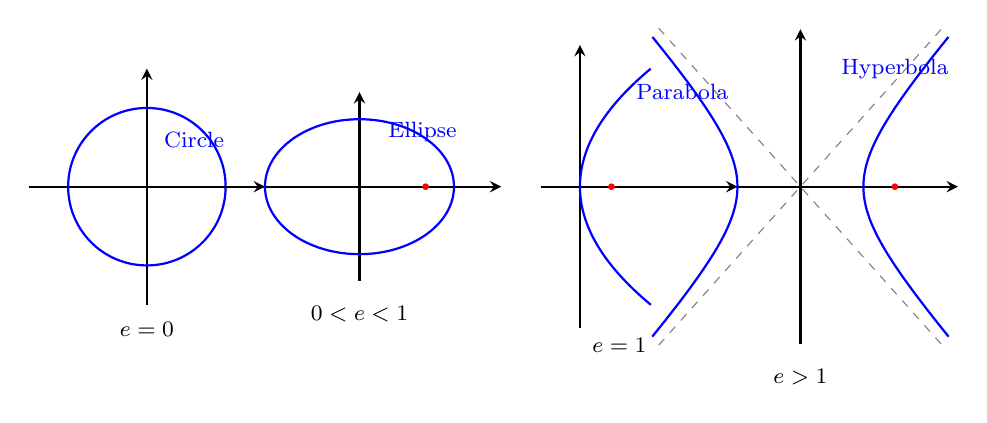
\begin{tikzpicture}[scale=1.0, >=stealth]
  % Four sub-figures for different eccentricities

  % --- e=0: Circle ---
  \begin{scope}[shift={(-4,0)}]
    \draw[->, thick] (-1.5,0) -- (1.5,0);
    \draw[->, thick] (0,-1.5) -- (0,1.5);
    \draw[blue, thick] (0,0) circle (1);
    \node[below, font=\footnotesize] at (0,-1.6) {$e=0$};
    \node[blue, font=\footnotesize] at (0.6, 0.6) {Circle};
  \end{scope}

  % --- e=0.7: Ellipse ---
  \begin{scope}[shift={(-1.3,0)}]
    \pgfmathsetmacro{\e}{0.7}
    \pgfmathsetmacro{\a}{1.2}
    \pgfmathsetmacro{\b}{\a*sqrt(1-\e*\e)}
    \pgfmathsetmacro{\c}{\a*\e}
    \draw[->, thick] (-1.8,0) -- (1.8,0);
    \draw[->, thick] (0,-1.2) -- (0,1.2);
    \draw[blue, thick] (0,0) ellipse ({\a} and {\b});
    \filldraw[red] (\c, 0) circle (1pt);
    \node[below, font=\footnotesize] at (0,-1.4) {$0 < e < 1$};
    \node[blue, font=\footnotesize] at (0.8, 0.7) {Ellipse};
  \end{scope}

  % --- e=1: Parabola ---
  \begin{scope}[shift={(1.5,0)}]
    \draw[->, thick] (-0.5,0) -- (2,0);
    \draw[->, thick] (0,-1.8) -- (0,1.8);
    \draw[blue, thick, domain=-1.5:1.5, samples=100]
      plot ({0.4*\x*\x}, \x);
    \filldraw[red] (0.4, 0) circle (1pt);
    \node[below, font=\footnotesize] at (0.5,-1.8) {$e=1$};
    \node[blue, font=\footnotesize] at (1.3, 1.2) {Parabola};
  \end{scope}

  % --- e=1.5: Hyperbola ---
  \begin{scope}[shift={(4.3,0)}]
    \pgfmathsetmacro{\e}{1.5}
    \pgfmathsetmacro{\a}{0.8}
    \pgfmathsetmacro{\b}{\a*sqrt(\e*\e-1)}
    \pgfmathsetmacro{\c}{\a*\e}
    \draw[->, thick] (-2,0) -- (2,0);
    \draw[->, thick] (0,-2) -- (0,2);
    \draw[blue, thick, domain=-1.5:1.5, samples=100]
      plot ({\a*cosh(\x)}, {\b*sinh(\x)});
    \draw[blue, thick, domain=-1.5:1.5, samples=100]
      plot ({-\a*cosh(\x)}, {\b*sinh(\x)});
    % Asymptotes
    \draw[dashed, gray, thin] (-1.8, {-\b/\a*1.8}) -- (1.8, {\b/\a*1.8});
    \draw[dashed, gray, thin] (-1.8, {\b/\a*1.8}) -- (1.8, {-\b/\a*1.8});
    \filldraw[red] (\c, 0) circle (1pt);
    \node[below, font=\footnotesize] at (0,-2.2) {$e > 1$};
    \node[blue, font=\footnotesize] at (1.2, 1.5) {Hyperbola};
  \end{scope}
\end{tikzpicture}
\end{document}
